\documentclass[handout]{beamer}

\usetheme[progressbar=frametitle]{metropolis}
\metroset{block=fill}

\subtitle{NTIN071 Automata and Grammars}
\author{Jakub Bulín (KTIML MFF UK)}

\date{Spring 2025\\ 
    \vspace{1in} 
    \begin{flushleft}
        \it \footnotesize * Adapted from the Czech-lecture slides by Marta Vomlelová with gratitude. The translation, some modifications, and all errors are mine.
    \end{flushleft}
}

%% packages

\usepackage{amsmath}
\usepackage{amssymb}
\usepackage{amsthm}
\usepackage{cancel}
\usepackage{color}
\usepackage{colortbl}
\usepackage{forest}
\usepackage[utf8x]{inputenc}
\usepackage{multicol}
\usepackage{multirow}

%% colors
\definecolor{Gray}{gray}{0.9}

%% TikZ
\usepackage{tikz}
    \usetikzlibrary{
        automata,
        arrows,
        backgrounds,
        decorations.pathmorphing,
        fit,
        positioning,
        shapes,
        shapes.geometric,
        tikzmark
    } 
    \tikzset{>=stealth',shorten >=1pt,auto,node distance=2cm}
    \tikzset{initial text={}}
    \tikzset{elliptic state/.style={draw,ellipse}}

%% amsthm
\theoremstyle{plain}
    \newtheorem*{algorithm}{Algorithm}    
    \newtheorem*{observation}{Observation}
    \newtheorem*{proposition}{Proposition}

\theoremstyle{remark}
    \newtheorem*{exercise}{Exercise}
    \newtheorem*{remark}{Remark}

%% macros
\DeclareMathOperator{\RegE}{RegE}
\DeclareMathOperator{\RL}{RL}

% Just for Lecture 2
\newcommand{\x}{$\times$}
\newcommand{\nx}{\ }



\title{Lecture 10 -- Turing Machines, Linear-bounded automata}


\begin{document}


\frame{\titlepage}


\begin{frame}{Recap of Lecture 9}
	
    \begin{itemize}        
        \item Closure properties of context-free languages (including substitution, homomorphism, inverse homomorphism)
        \item Also closure properties of deterministic CFLs
        \item Dyck languages, a characterization of context-free languages
    \end{itemize}
	
\end{frame}


\section{\sc Chapter 3: Turing Machines}


\section{3.1 Turing machine}


\begin{frame}{History and motivation}
    
    1931--1936 Gödel, Church, Turing, Kleene: formalize \alert{`algorithms'}
    
    \smallskip
    
    \alert{Turing machine}: a general model of any computer
    \begin{itemize}
        \item a two-way infinite \alert{tape} (sequential memory)
        \item a \alert{head} to read/write, moves in both directions
        \item a control unit (finite state)
    \end{itemize}
    \vspace{-9pt}
    \begin{center}
        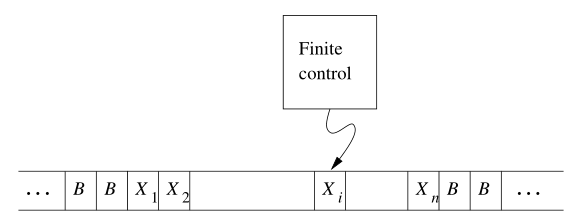
\includegraphics[width=0.8\textwidth]{files/tm1.PNG}  
    \end{center}        
    \vspace{-9pt}
    Other formalizations: RAM, $\lambda$-calculus, partially recursive functions

    \alert{Computability theory}: what problems can['t] computers solve?

\end{frame}


\begin{frame}{The definition}

    A \alert{Turing Machine (TM)} is $M=(Q,\Sigma,\Gamma,\delta,q_0,B,F)$ where:
    
    \begin{itemize}
        \item $Q$ is a finite, nonempty set of \alert{states}
        \item $\Sigma$ is a finite, nonempty \alert{input alphabet} 
        \item $\Gamma$ is a finite, nonempty \alert{tape alphabet}, $\Gamma \supseteq \Sigma$, $Q\cap \Gamma=\emptyset$
        \item $\delta\colon(Q\setminus F)\times\Gamma\rightarrow Q\times \Gamma\times \{L,R\}$ is the (partial) \alert{transition function}, i.e., one instruction is $\delta(q,x)=(p,Y,D)$ where:
        \begin{itemize}
            \item $q\in Q\setminus F$ is the current state [no transitions out of final states]
            \item $X\in\Gamma$ is the tape symbol in the current cell
            \item $p\in Q$ is the next state to switch to
            \item $Y\in \Gamma$ is the tape symbol to rewrite $X$ with in the current cell
            \item $D\in \{L,R\}$ is the \alert{direction} in which the head then moves
        \end{itemize}
        \item $q_0\in Q$ is the \alert{start state}
        \item $B\in\Gamma\setminus\Sigma$ is the \alert{blank symbol}, initially written in all but finitely many cells that hold the input symbols
        \item $F\subseteq Q$ are the \alert{final} or \alert{accepting} states
    \end{itemize}

\end{frame}


\begin{frame}{Describing computation: configurations}

    \textbf{Recall} \alert{computation graph}: vertices=\alert{configurations}, arcs=\alert{moves}~$\vdash$


    A \alert{configuration} of a TM is a finite string 
    $$
    X_1X_2\ldots X_{i-1}qX_iX_{i+1}\ldots X_n
    $$

    \begin{itemize}
        \item $q\in Q$ is the current state
        \item $X_1\ldots X_n\in\Gamma^*$ describe the contents of the relevant portion of the tape, that is, between
        \begin{itemize}
            \item the first (leftmost) non-blank symbol or head position, and
            \item the last (rightmost) non-blank symbol or head position
        \end{itemize} 
        \item the tape head is scanning the $i$-th symbol $X_i\in\Gamma$
    \end{itemize}
    
\end{frame}


\begin{frame}{Describing computation: moves}

    For \alert{moves} of a TM $M$, use same notation as for PDA: $\vdash_M, \vdash_M^*, \vdash^*$
    
    \medskip

    \begin{itemize}
        \item For $\delta(q,X_i)=(p,Y,L)$: 
        $$
        X_1X_2\ldots X_{i-1}qX_iX_{i+1}\ldots X_n \vdash_M X_1X_2\ldots X_{i-2}pX_{i-1}\textbf{Y}X_{i+1}\ldots X_n
        $$
        \item For $\delta(q,X_i)=(p,Y,R)$: 
        $$
        X_1X_2\ldots X_{i-1}qX_iX_{i+1}\ldots X_n \vdash_M X_1X_2\ldots X_{i-1}\textbf{Y}pX_{i+1}\ldots X_n
        $$
    \end{itemize}

    \medskip

    And $\vdash_M^*$ is a reflexive, transitive closure of $\vdash_M$ (oriented \alert{path} in the computation graph).

    \medskip

    \alert{initial configuration:} $q_0w$ for the input word $w\in\Sigma^*$\\
    \alert{accepting configurations:} those where $q\in F$, any tape contents (i.e., in our definition, the TM doesn't need to `clean' the tape)

\end{frame}


\begin{frame}{The language, an example}

    The language \alert{recognized by} a TM $M=(Q,\Sigma, \Gamma, \delta,q_0,B,F)$ is:    
    $$
    \alert{L(M)}=\{w\in \Sigma^*\mid q_0w \vdash_M^* \alpha p \beta, p\in F, \alpha,\beta \in \Gamma^*\}
    $$
    A language is \alert{recursively enumerable} if it is recognized by some TM

    \bigskip

    \begin{example}
        The following TM accepts the language $L=\{0^n1^n\mid n\geq 1\}$:
        $$
        M=(\{q_0,q_1,q_2,q_3,q_4\},\{0,1\},\{0,1,X,Y,B\},\delta,q_0,B,\{q_4\})
        $$

        \vspace{-15pt}
        \begin{center}
            \small
            \begin{tabular}{c | c c c c c}
            $\delta$ & $0$ & $1$ & $X$ & $Y$ & $B$\\
            \hline \hline
            $q_0$ & $(q_1,X,R)$& -- & -- & $(q_3,Y,R)$& --\\
            $q_1$ & $(q_1,0,R)$& $(q_2,Y,L)$& -- & $(q_1,Y,R)$& --\\
            $q_2$ & $(q_2,0,L)$& -- & $(q_0,X,R)$& $(q_2,Y,L)$& --\\
            $q_3$ & -- & -- & -- & $(q_3,Y,R)$& $(q_4,B,R)$\\
            $q_4$ & -- & -- & -- & -- & --
            \end{tabular}
        \end{center}
        \vspace{-9pt}
    \end{example}

\end{frame}


\begin{frame}{Transition diagram}

    \vspace{-6pt}
    \alert{nodes} are states, \alert{arcs} $q\to p$ are labeled by $X/YD$ for all $\delta(q,X)=(p,Y,D)$ (use $D\in\{\leftarrow,\rightarrow\}$ instead of $\{L,R\}$)
    
    \vspace{-3pt}
    \begin{center}
        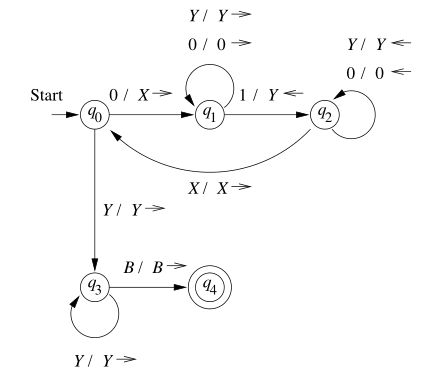
\includegraphics[width=0.72\textwidth]{files/tmTrans.PNG}
    \end{center}
    
\end{frame}


\begin{frame}{The program explained}

    
\end{frame}


\begin{frame}{Computation: examples}
    
       
    $w=0011$

    $$q_00011\vdash Xq_1011\vdash X0q_111\vdash Xq_20Y1\vdash q_2X0Y1\vdash Xq_00Y1\vdash 
    XXq_1Y1\vdash 
    $$    
    $$
    \vdash XXYq_11\vdash XXq_2YY \vdash  Xq_2XYY\vdash XXq_0YY\vdash XXYq_3Y\vdash XXYYq_3B\vdash XXYYBq_4B
    $$
    
    $w=0010$

    $$
    q_00010\vdash Xq_1010\vdash X0q_110\vdash Xq_20Y0\vdash q_2X0Y0\vdash Xq_00Y0\vdash 
    XXq_1Y0\vdash
    $$
    $\vdash XXYq_10\vdash XXY0q_1B$ ends in failure, because there is no instruction
    
\end{frame}




\section{3.2 Variants of TMs}


\section{3.3 TMs and grammars}


\end{document}


